\subsection{HTML}
\label{html}\index{HTML}
\ac{html} dient als Sprache, um HTML-Dokumente zu beschreiben. Ein HTML-Dokument\index{HTML-Dokument} ist ein Textdokument, bestehend aus mehreren Tags\index{Tag}. Dies sind in spitzen Klammern eingeschlossene Namen. Sie können durch Attribute weiter beschrieben werden. Ein Tag beschreibt Texte, Überschriften, Bilder, Tabellen etc. Zudem können Tags ineinander verschachtelt werden, um zusammenhängende Elemente logisch zu gruppieren. Ein Webbrowser\index{Webbrowser} kann diese Struktur interpretieren und entsprechend darstellen \cite{lub07}. Die aktuelle Version HTML5\index{HTML!HTML5} wurde am 28.10.2014 veröffentlicht und bietet einige neue Funktionen \cite{W3C2014}. Der typische Aufbau eines HTML-Dokumentes\index{HTML!HTML-Dokument} ist hierbei wie folgt.

\begin{lstlisting}[style=htmlcssjs, caption=Beispiel eines HTML-Dokumentes, label=lst:html]
<!DOCTYPE html>
<html>
  <head>
    <title>Der Seitentitle</title>
  </head>
  <body>
    <h1>Hello World</h1>
    <div id="inhalt">Meine erste Webseite!</div>
    <img src="flowerpot.png" alt="Eine Blume"/>
  </body>
</html>
\end{lstlisting}

Ein Webbrowser ist nun in der Lage den HTML-Code zu interpretieren und darzustellen, \autoref{lst:html} würde dabei wie \autoref{img:html} im Webbrowser aussehen.

\begin{figure}[H]
    \begin{center}
        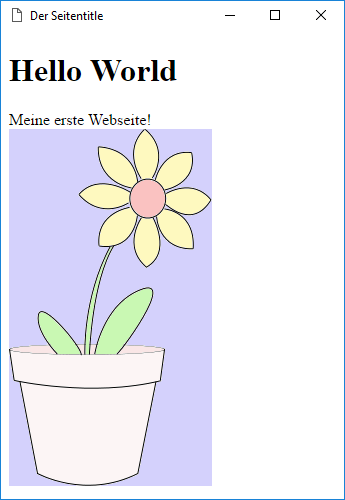
\includegraphics[width=.5\textwidth]{html.png}
        \caption{Beispiel HTML-Dokument im Browser angezeigt}
        \label{img:html}
    \end{center}
\end{figure}